Il seguente codice MatLab contiene la soluzione del problema dell'Es.7 :\\\
	\lstinputlisting[language=Matlab]{Cap_4/Es_7/Es_7.m}
La seguente figura mostra il polinomio \textit{p(x)}, interpolante le ascisse di Chebyshev, per la funzione di Runge \textit{f(x)}, al variare del grado \textit{N} del polinomio con $N=2,4,6,8...40$ :\\\
	\begin{figure}[H]
  		\label{Cap_4_Es_7}
  		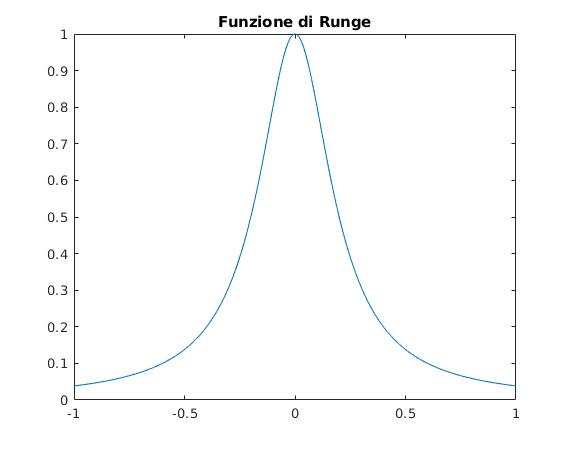
\includegraphics[width=\textwidth]{Plot/Cap_4_Es_7}
	\end{figure}
La seguente tabella mostra, la stima dell'errore al variare di N (grado del polinomio interpolante) tramite la norma euclidea 
della differenza tra i valori della funzione di \textit{Runge} e quelle del polinomio di \textit{Lagrange}:
	\begin{center}
		\begin{tabular}{|c|c|}
			\hline
				N & $\|f(x)-y\|$ \\
    			\hline
    				$2$  & $65.1749$ \\
    				$4$  & $51.8929$ \\
    				$6$  & $44.2988$ \\
    				$8$  & $39.3066$ \\
    				$10$ & $35.6975$ \\
    				$12$ & $32.9190$ \\
    				$14$ & $30.7265$ \\
    				$16$ & $28.8977$ \\
    				$18$ & $27.3972$ \\
    				$20$ & $26.0781$ \\
    				$22$ & $24.9797$ \\
   					$24$ & $23.9751$ \\
    				$26$ & $23.1381$ \\
    				$28$ & $22.3469$ \\
    				$30$ & $21.6900$ \\
    				$32$ & $21.0518$ \\
    				$34$ & $20.5221$ \\
    				$36$ & $20.0008$ \\
    				$38$ & $19.5675$ \\
    				$40$ & $19.1448$ \\
				\hline
		\end{tabular}
	\end{center} 